\documentclass[12pt]{article}

\usepackage[a4paper, margin=2cm]{geometry}
\usepackage{amsmath}

\usepackage{tikz}
\usepackage{tikz-feynman}
\tikzfeynmanset{compat=1.1.0}

\begin{document}

\section*{Beta-minus decay (time upwards, both leptons forward in time)}

\[
n \rightarrow p + e^- + \bar{\nu}_e
\]

\begin{center}
\begin{tikzpicture}
\begin{feynman}
  % Vertices (manual placement)
  \vertex (n)  at (0,0)   {\(n\)};
  \vertex [coordinate] (a)  at (1,2)   {};
  \vertex (p)  at (0,4) {\(p\)};

  \vertex [coordinate] (b)  at (4,2)   {};
  \vertex (e)  at (5,4) {\(e^-\)};
  \vertex (nu) at (6,3) {\(\bar{\nu}_e\)};

  \diagram*{
    (n) -- [fermion] (a) -- [fermion] (p),
    (a) -- [boson, edge label=\(W^-\), momentum'={}] (b),
    (b) -- [fermion] (e),
    (b) -- [fermion] (nu),
  };
\end{feynman}
\end{tikzpicture}


\begin{tikzpicture}
\begin{feynman}
  % Vertices
  \vertex (W) at (0,2) {};
  \vertex [coordinate] (v) at (3,2) {};

  \vertex (mu) at (4,4) {\(\mu^-\)};
  \vertex (nu) at (5,3) {\(\bar{\nu}_\mu\)};

  \diagram*{
    (W) -- [boson, edge label=\(W^-\), momentum'={}] (v),
    (v) -- [fermion] (mu),
    (v) -- [fermion] (nu),
  };
\end{feynman}
\end{tikzpicture}

\begin{tikzpicture}
\begin{feynman}
  % Left (hadronic) side
  \vertex (p)  at (0,0) {\(p\)};
  \vertex [coordinate] (a) at (1,2) {};
  \vertex (n)  at (0,4) {\(n\)};

  % Right (leptonic) side
  \vertex (e)  at (5,0) {\(e^-\)};
  \vertex [coordinate] (b) at (4,2) {};
  \vertex (nu) at (5,4) {\(\nu_e\)};

  \diagram*{
    (p) -- [fermion] (a) -- [fermion] (n),
    (a) -- [boson, edge label=\(W^+\), momentum'={}] (b),
    (e) -- [fermion] (b) -- [fermion] (nu),
  };
\end{feynman}
\end{tikzpicture}


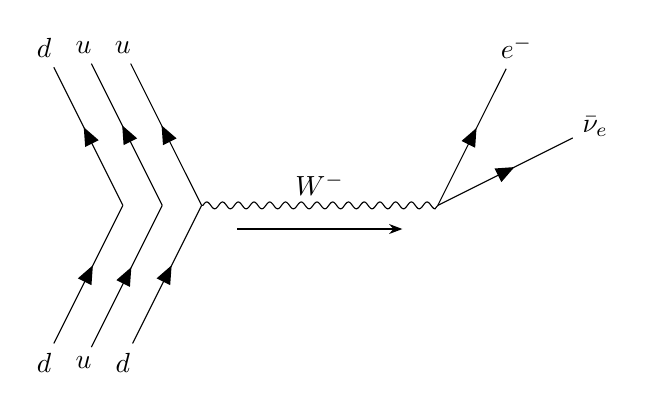
\begin{tikzpicture}
\begin{feynman}
  % Spectator Quarks
  \vertex (l4)  at (-1,0)   {\(d\)};
  \vertex [coordinate] (c)  at (0,2)   {};
  \vertex (l3)  at (-1,4) {\(d\)};

  \vertex (l6)  at (-0.5,0)   {\(u\)};
  \vertex [coordinate] (d)  at (0.5,2)   {};
  \vertex (l5)  at (-0.5,4) {\(u\)};

  % Participating Quarks
  \vertex (l2)  at (0,0)   {\(d\)};
  \vertex [coordinate] (a)  at (1,2)   {};
  \vertex (l1)  at (0,4) {\(u\)};

  \vertex [coordinate] (b)  at (4,2)   {};
  \vertex (r1)  at (5,4) {\(e^-\)};
  \vertex (r2) at (6,3) {\(\bar{\nu}_e\)};

  \diagram*{
    (l4) -- [fermion] (c) -- [fermion] (l3),
    (l6) -- [fermion] (d) -- [fermion] (l5),
    (l2) -- [fermion] (a) -- [fermion] (l1),
    (a) -- [boson, edge label=\(W^-\), momentum'={}] (b),
    (b) -- [fermion] (r1),
    (b) -- [fermion] (r2),
  };
\end{feynman}
\end{tikzpicture}

\begin{tikzpicture}
\begin{feynman}
  % Vertices
  \vertex (l1) at (0,0) {\(d\)};
  \vertex [coordinate] (a) at (1,2) {};
  \vertex (l2) at (0,4) {\(u\)};
  \vertex (b) at (4,2) {};

  \diagram*{
    (l1) -- [fermion] (a) -- [fermion] (l2),
    (a) -- [boson, edge label=\(W^-\), momentum'={}] (b),
  };
\end{feynman}
\end{tikzpicture}


\end{center}
\end{document}
